\documentclass[mscThesis.tex]{subfiles}

\begin{document}

\chapter{Introduction}
\label{chap:Int}
%background
%general robotics
Robotic systems are widely used in industry nowadays. The use of robots in various applications instead of humans can lead to improvements both in terms of costs and task performance. Robotic systems show their use mostly in applications that are so-called ``4D tasks'', tasks that are dangerous, dull, dirty or dumb \cite{wtec2006}. A common property of the 4D tasks is that the robots are used in a repetitive setting: the same exact task is performed repeatedly. Examples of common robotic tasks can be found in material handling, such as welding or 3D printing. The human interaction with such a robot is often not allowed during operation. Usually, a cage is present to guarantee the safety of employees that are present. When using robots in this environment, it makes sense to program each robotic task manually. It allows the programmer to optimize the robot for each task. For example, a robot could be programmed to perform a task as fast a possible, for maximum production speed. Therefore, manual implementation of robotic tasks is still the most used practice in the industrial application of robots \cite{biggs2003survey}.

%Issue: control. Robot hardware is good enough usually
There are two aspects of the manual programming approach that are prone for improvement. First off, the process of programming a robotic task is expensive and time consuming. The cost of robotic experts makes the use of robots economically unfeasible for small series of tasks, especially tasks outside 4D area. Furthermore, the controllers that result from this process generalize very poorly. In a different environment the robot will not perform as well, it has to be tuned again. Also if the application of the robot operates in a dynamic environment, such as a human-robot interaction task, a more adaptive control strategy is needed.

% Reinforcement learning
Several control strategies have been developed that focus on the control of environments that change over time. One of these methods called Reinforcement Learning (RL), has interesting properties for robotic applications. Reinforcement learning methods can operate dynamic and noisy environments without the need of a model \cite{SuttonBarto1998}. The RL method also applies optimization to achieve its pre-defined purpose \cite{Lewis2009}. An important element of the RL algorithm, the reward function, defines the assignment that the robot has to execute. In many applications, this reward function is defined by the programmer and tuned manually to produce the best result. This form of manual programming is still expensive and time consuming. Also, for many tasks, a measure of success is hard to define explicitly. 

A simple example in Figure \ref{fig:example-task} illustrates how a RL algorithm converges to a different outcome than originally intended. The task, which is intended by the programmer, is from the end effector of a robot arm to move from an initial position towards a goal. In between it should pass through a point in space. As can be seen from the final trajectory, the end effector passes the viapoint with precision. However, the path towards the viapoint can be described as an inefficient detour. The problem in this example is that the reward function, which is the RL equivalent of the cost function used in optimal control, is defined too simple. 

\begin{figure}
\centering
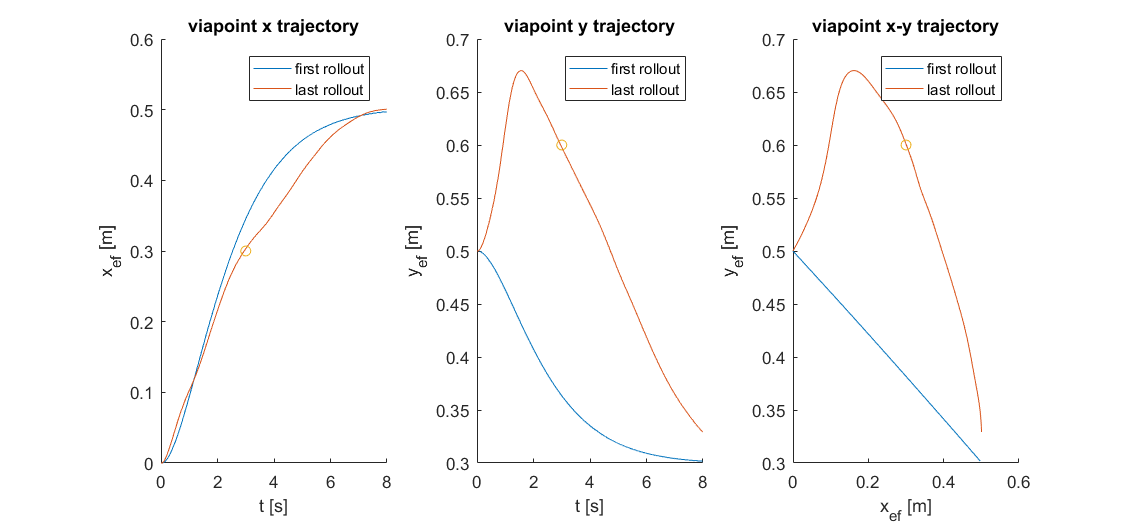
\includegraphics[width=\textwidth, keepaspectratio=1]{figures/trajectory-static-via.png}
\caption{Resulting trajectories of a simple via point task.}
\label{fig:example-task}
\end{figure}

% Active reward learning
A better alternative would be to teach the robot a task from another entity, called the expert, that knows exactly how the task needs to be performed. There are several approaches that accomplish machine learning from an expert. In the field of reinforcement learning, two approaches have been studied extensively: Apprenticeship learning and Inverse Reinforcement Learning (IRL). Both methods rely extensively on the availability of example (sub-) optimal trajectories, supplied by the expert. Inverse reinforcement learning differs from apprenticeship learning by the notion that IRL methods try to obtain the underlying reward function where apprenticeship learners try to obtain the optimal policy. The former class of methods is more interesting as an approach for adaptive control, because the obtained reward function can be used in different environments. 

A more recent method is the Active Reward Learning method (ARL) \cite{Daniel2015}. The idea of active reward learning is similar to inverse reinforcement learning as this method also constructs a reward function, using the expert as source of information. In this setting, the expert is used to give feedback on robot trajectories. Active reward learning has been applied to a small number of robotic problems. The experiments in \cite{Daniel2015} show how ARL can be applied to an inverse learning problem. In this experiment, the robot learns how to cross a viapoint in Cartesian space by controlling motor commands in joint space. As input for the reward function the robot is given the difference between the position of the end effector and the viapoint. As a result, a reward model containing a squared relation with respect to the viapoint error is returned. In a more advanced experiment, a robot hand is taught how to grab an unknown object, based on the calculated forces at the fingertips. 

\section{Task description}
In this thesis we adopt the task description of the first experiment in \cite{Daniel2015}, which is a viapoint task, as we would like to improve on this work. The viapoint task is described as follows: Given an initial position $\bm{x}_{\text{init}}$, goal position $\bm{x}_{\text{goal}}$ and a viapoint $\bm{x}_{\text{viapoint}}$ in Cartesian space, construct a path in Cartesian space such that the end effector of a robot arm travels from $\bm{x}_{\text{init}}$ to $\bm{x}_{\text{goal}}$, crossing $\bm{x}_{\text{viapoint}}$ at a specific point in time $t_{\text{viapoint}}$. An example of such a task in is on display in Figure \ref{fig:viapoint-example}. In all experiments conducted, we assume the trajectories to be of fixed length $t_N$ in discrete time.

A second task that we use in the experiments, which is very similar to the viapoint task, is a viaplane task. Similar to the viapoint task, during a viaplane experiment, the end effector of a robotic arm needs to travel from $\bm{x}_{\text{init}}$ to $\bm{x}_{\text{goal}}$ in Cartesian space. However, instead of crossing a single point in between $\bm{x}_{\text{init}}$ and $\bm{x}_{\text{goal}}$, the end effector has to cross a pre-defined plane in a specific region in the time line. Such a task can be combined with a viapoint task to generate a more challenging goal for the robot arm to achieve, as is shown in Figure \ref{fig:viaplane-example}. 

\begin{figure}[!htb]
    \centering
    \begin{minipage}{.5\textwidth}
        \centering
        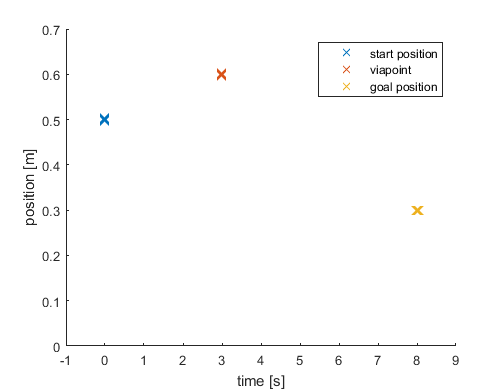
\includegraphics[width=0.8\linewidth, keepaspectratio]{figures/example-viapoint}
        \caption{Viapoint task in one dimension.}
        \label{fig:viapoint-example}
    \end{minipage}%
    \begin{minipage}{0.5\textwidth}
        \centering
        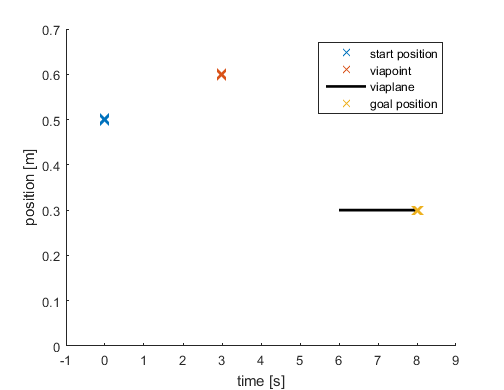
\includegraphics[width=0.8\linewidth, keepaspectratio]{figures/example-viaplane}
        \caption{Viaplane in combination with viapoint task in one dimension.}
        \label{fig:viaplane-example}
    \end{minipage}
\end{figure}

The combination of viapoints and viaplanes can be used to define various end effector movements. For example, we can teach a robot arm to move towards a known goal and avoid an area with obstacles. Also, we can teach the robot to approach the end goal from a certain angle. This technique can be used for example to teach the robot an insertion task.


In this thesis, a simulated 2 degrees-of-freedom robotic arm is used for conducting experiments. In all tests, the algorithm is used to define a path in Cartesian end effector space, so the reinforcement learning agent will define a path in $x$ and $y$ coordinates. In order to convert this trajectory into a set of motor commands, an inverse kinematics block is needed as can be seen in Figure \ref{fig:overview-ARL-robot}. This block will effectively convert the path defined in Cartesian space to joint space using the Jacobian method. After performing a rollout of the simulator, the resulting trajectory in joint-space is converted back to Cartesian space using a forward kinematics block. After the forward kinematics conversion, the resulting trajectory in Cartesian space is used for evaluating the policy. 


\begin{figure}[!ht]
\centering
\begin{tikzpicture}[->, >=stealth']

\node[state,
        minimum width = 11cm,
        minimum height = 2cm] (ARL) {
	ARL
 };

\node[	state,
		below of= ARL,
		node distance = 0cm,
		xshift = -4cm,
		text width = 2 cm,
		] (policy) {
 	policy
 };
 
\node[	state,
		below of = ARL, xshift = 4cm,
		node distance = 0cm,
		text width = 2.5 cm,
		] (reward)  { 
    reward model
 }; 
 
\node[ 	state,
		below of = policy,
		text width = 2 cm,
		node distance = 4 cm
		] (ik) {
	IK
 };
 
\node[ 	state,
		right of = ik,
		text width = 2 cm,
		node distance = 4 cm] (arm) {
	robot arm
 };
 
\node[ 	state,
		right of = arm,
		text width = 2 cm,
		node distance = 4 cm
		] (fk) {
	FK
 };
 
  
\path 	
 		(policy) 	edge 						
 					node[text width = 3 cm]	
 						{\small Cartesian input trajectory}
 												(ik)
 		(ik) 		edge
 		 			node[	anchor = south,
 		 					text width = 2 cm]	
 						{\small joint input trajectory}
 						 						(arm)						
 		(arm)		edge
 		 			node[	anchor = south,
 		 					text width = 2 cm]	
 						{\small joint output trajectory}
 						 						(fk)
 		(fk)		edge
 		 			node[text width = 3 cm]	
 						{\small Cartesian output trajectory}
 						 						(reward);
 		
\end{tikzpicture}
\caption{Overview of the interaction between the robot and the ARL algorithm.}
\label{fig:overview-ARL-robot}
\end{figure}

\section{Research goals}
\label{sec:research-goals}
% purpose
Although the ARL method has been proven to work in a practical example, there is room for more research. This thesis investigates two options for improving the viapoint experiment conducted in \cite{Daniel2015}. First off, the input of the reward model constructed in \cite{Daniel2015} contains information about the exact position of the viapoints and time slot at which the end effector should cross it and this is usually absent in practical cases. We will come up with a method that is able to learn viapoints in Cartesian space purely based on expert feedback. As input for the reward model we will construct features that does not contain any task-specific information. 

One major problem in this more realistic approach is that the reward model will lack information about which points in time are important to focus on. In order to alleviate this problem, we introduce a segmentation on the time line of robot trajectories. It is possible, by adapting the input definitions of the reward model, to use the ARL algorithm introduced in \cite{Daniel2015} and apply it in such a way that we are able to learn time segmented active reward learning. 

This adaptation of ARL still considers that the human expert is only able to give a rating over full trajectories. The amount of information that the expert gives is limited to one grade per complete trajectory. We could extend this framework such that the expert can give feedback on time segments of the trajectory. A more sophisticated adaptation on the ARL algorithm, which basically constructs a different reward model for each time segment, is needed to achieve this kind of time segmented learning. The hypothesis is that with this new source of expert information, the accuracy of the end effector trajectories will improve.

The purpose of this thesis is to show the results of two time segmented ARL algorithms. In this experiment we try to answer the following research questions: 

\begin{itemize}
\item Can we use time segmented active reward learning to teach a robotic arm a simple viapoint task? Is it possible to learn more complicated trajectories using time segmented active reward learning?
\item How many expert queries are necessary to achieve convergence for a viapoint task on a robotic arm, using time segmented active reward learning? Does the time segmentation make a difference in expert queries needed? Is this number of expert queries within the limits of practical application? 
\item How many roll outs are needed to learn a viapoint task with a time segmented reward model compared with a full-trajectory reward model? Is the number of roll outs of the time segmented algorithm within practical limits? 
\end{itemize}


\section{Roadmap}
In order to give an overview of the contents of this work, a roadmap is provided in Figure \ref{fig:roadmap}. The order of subjects is best explained when we take a brief look at the general formulation of reward learning.
%
As shown in semi-mathematical Equation \eqref{eq:double-opt}, active reward learning is essentially solving a double optimization problem. The main goal is to maximize the expert ratings through querying demonstrated rollouts. We can adjust the reward function in order to accomplish better results from the reinforcement learning agent. These results flow from the second optimizer, which is a straight-forward RL problem.

\begin{equation}
\underbrace{\max_{\text{reward function}} \text{expert} \overbrace{ \left(  \max_{\text{policy}} \text{reward function} (\text{policy}) \right) }^{\text{Reinforcement learning (Chapter \ref{chap:RL})}}   }_\text{Reward learning (Chapters \ref{chap:Reward}-\ref{chap:SARL})}
\label{eq:double-opt}
\end{equation}

%Layout
In Chapter \ref{chap:RL}, we will focus on the second optimizer, the forward RL method. We will review the RL methods that are applied to continuous systems as this is the application that we are focusing on. One specific reinforcement learning method will be described in more detail, as this method will be used in Chapters \ref{chap:ARL}-\ref{chap:SARL} as well. After that, two different approaches to reward learning are explained in Chapter \ref{chap:Reward}, namely inverse reinforcement learning and active reward learning. We will explain the difference between the two methods and discuss the advantages and disadvantages of both methods in detail. In Chapter \ref{chap:ARL}, the active reward learning method is described in more detail. Also, we will show how we can use ARL to teach a viapoint task to a robotic arm. After that, in Chapter \ref{chap:SARL}, an extension to the active reward learning algorithm, called segmented active reward learning is introduced. After a theoretical introduction to this new variant of ARL, we will show the results of this new method in Chapter \ref{chap:Ex} and compare them to the original ARL method. At last we will review the results of the research and show some recommendations for further research. 

\begin{figure}[!ht]
\centering
\begin{tikzpicture}[->,>=stealth']

 % Position of QUERY 
 % Use previously defined 'state' as layout (see above)
 % use tabular for content to get columns/rows
 % parbox to limit width of the listing
 \node[	state,
 		text width = 3.5 cm] (CHAPTER1) {
 
	\begin{tabular}{l}
  		\textbf{\small Chapter 1}\\
  		\parbox{3 cm} {\small Introduction}
 	\end{tabular} 
 };
 
 \node[	state,
 		text width = 3.5 cm,
 		below of = CHAPTER1,
 		node distance = 2 cm
 		] (CHAPTER2) {
 
	\begin{tabular}{l}
  		\textbf{\small Chapter 2}\\
  		\parbox{3 cm} {\small Reinforcement Learning}
 	\end{tabular} 
 };
 
  \node[	state,
 		text width = 3.5 cm,
 		below of = CHAPTER2,
 		node distance = 2 cm
 		] (CHAPTER3) {
 
	\begin{tabular}{l}
  		\textbf{\small Chapter 3}\\
  		\parbox{3 cm} {\small Reward Learning}
 	\end{tabular} 
 };
 
   \node[	state,
 		text width = 3.5 cm,
 		below of = CHAPTER3,
 		node distance = 2 cm
 		] (CHAPTER4) {
 
	\begin{tabular}{l}
  		\textbf{\small Chapter 4}\\
  		\parbox{3 cm} {\small Active Reward Learning}
 	\end{tabular} 
 };
 
  \node[	state,
 		text width = 3.5 cm,
 		below of = CHAPTER4,
 		node distance = 2cm
 		] (CHAPTER5) {
 
	\begin{tabular}{l}
  		\textbf{\small Chapter 5}\\
  		\parbox{3 cm} {\small Segmented Active Reward Learning}
 	\end{tabular} 
 };
 
  \node[	state,
 		text width = 3.5 cm,
 		below of = CHAPTER5,
 		node distance = 2cm
 		] (CHAPTER6) {
 
	\begin{tabular}{l}
  		\textbf{\small Chapter 6}\\
  		\parbox{3 cm} {\small Experiment results}
 	\end{tabular} 
 };
 
 \path  
 	(CHAPTER1) edge (CHAPTER2)
 	(CHAPTER2) edge (CHAPTER3)
 	(CHAPTER3) edge (CHAPTER4)
 	(CHAPTER4) edge (CHAPTER5)
 	(CHAPTER5) edge (CHAPTER6);
 	
 	\draw [dashed, ->]

		(CHAPTER2.east)
		-- ++(0.5, 0)
		|- (CHAPTER4.east);
 

\end{tikzpicture}
\caption{Roadmap of the report. The dashed line represents an a shortcut through the material.}
\label{fig:roadmap}
\end{figure}

% Bibliography
%\bibliographystyle{ieeetr}
%\printbib{bibliography}
%

\end{document}